%%%%%%%%%%%%%%%%%%%%%%%%%%%%%%%%%%%%%%%%%%%%%%%%
% Vektorgeometrie
%%%%%%%%%%%%%%%%%%%%%%%%%%%%%%%%%%%%%%%%%%%%%%%%
\section{Vektorgeometrie}

\subsection{Gerade}
	Parametergleichung: \begin{tabular}{ll}
		& $\vec{p_0} = $ Stützvektor \\
		$g = \lbrace\vec{p_0} + t\vec{r} | t \in \mathbb{R}\rbrace$ & $\vec{r} = $ Richtungsvektor \\
		& $t = $ Paramter
	\end{tabular}

	\subsubsection{Punkt auf Geraden}
		$\vec{q} = \vec{p_0} + t\vec{r} \Longrightarrow \begin{array}{|c|c|}
			\hline r_1 & q_1 - p_{01}\\
			\hline r_2 & q_2 - p_{02}\\
			\hline \end{array} \rightarrow^{Gauss} 
		\begin{array}{|c|c|}
			\hline 1 & * \\
			\hline 0 & \color{red}*\\
			\hline \end{array}$ \qquad 
		\begin{tabular}{l}
			${\color{red}*} \neq 0 \Rightarrow$ keine Lösung\\
			${\color{red}*} = 0 \Rightarrow$ $t$ eindeutig; $t$ durch erste Gleichung ausrechnen
		\end{tabular}
	
	\subsubsection{Schnittgerade}
		Beide Geraden gleichsetzen und nach $t$ auflösen $\left\lbrace\begin{array}{l}
			\text{regulär: } t \text{ ist eindeutig}\\
			\text{singulär: } \left\lbrace\begin{array}{l}
				\infty \text{ Lösungen } \rightarrow \text{ Geraden liegen aufeinander}\\
				0 \text{ Lösungen } \rightarrow \text{ Geraden sind parallel}
			\end{array}\right.
		\end{array}\right.$


\subsection{Ebene}
	Parametergleichung: \begin{tabular}{ll}
		& $\vec{p_0} =$ Stützvektor\\
		$\tau = \lbrace\vec{p_0} + t_1\vec{r_1} + t_2\vec{r_2} | t_1, t_2 \in \mathbb{R}\rbrace$ & $\vec{r_1}, \vec{r_2} =$ Spannvektoren \\
		& $t_1, t_2 =$ Paramter
	\end{tabular}

	\subsubsection{Hessche Normalform}
		$ax + by + cz - d = 0$\\
		$\vec{n_0} \bullet (\vec{p} - d) = 0$\\
		$d = \vec{p_0} \bullet \vec{n_0} = \vec{p_0} \bullet \frac{\vec{n}}{|\vec{n}|} \qquad \qquad
		d = $ Abstand von Nullpunkt zu Ebene wenn $\left|\vektor{a}{b}{c}\right| = 1$ (Länge/Betrag)

	\subsubsection{Speziallfälle der Koordinatengleichung}
		\begin{tabular}{ll}
			$a = 0 \Rightarrow by + cz = d$ & Ebene ist parallel zur $x$-Achse (äguivalent bei b und c)\\
			$a = b = 0 \Rightarrow cz = d$ & Ebene ist parallel zur $x$ und $y$- Koordinatenebene\\
			$d = 0 \Rightarrow ax + by + cz = 0$ & Ebene enthält Ursprung 0 des Koordinatensystems
		\end{tabular}

	\subsubsection{Achsenabschnittgleichung der Ebene}
		Beispiel: $\tau = 3x + 6y + 4z = 18 \Leftrightarrow \frac{3a + 6y + 4z}{18} = 1 \Leftrightarrow \frac{3}{18}x + \frac{6}{18}y + \frac{4}{18}z = 1
		\Leftrightarrow \frac{x}{6} + \frac{y}{3} + \frac{z}{4.5} = 1$\\
		Die Achsenabschnitte der Ebene $\tau$ liegen nun bei $x = 6, y = 3, z = 4.5$.\\
		Allgemeine Achsenabschnittgleichung: $$ \frac{x}{p_x} + \frac{y}{p_y} + \frac{z}{p_z} = 1$$

\subsection{Kreis und Kugel}
	Parametergleichung: \begin{tabular}{ll}
		& $\vec{m} =$ Mittelpunkt \\
		$K(M,r) = \lbrace (\vec{p} - \vec{m}) \cdot (\vec{p} - \vec{m}) = r^2 \rbrace$ & $\vec{p} =$ Punkt am äusseren Rand\\
		& $r =$ Radius
	\end{tabular}\\

	\begin{equation*}
		(\vec{p} - \vec{m})^2 = r^2  \qquad \Leftrightarrow \qquad (p_1 - m_1)^2 + (p_2 - m_2)^2 + (p_3 - m_3)^2 = r^2
	\end{equation*}

	\subsubsection{Tangentialebene}
		\begin{tabular}{lll}
			$(\vec{p_0} - \vec{m})(\vec{p} - \vec{p_0}) = 0$ & & $\vec{p_0} =$ Berührpunkt\\
			$r \cdot (\vec{p} - \vec{p_0}) = 0$ & & $\vec{p} =$ Punkt auf der Tangente\\
			$(\vec{p_0} - \vec{m})^2 = r^2$ & & $\vec{m} =$ Mittelpunkt des Kreises/Kugel
		\end{tabular}

	\subsubsection{Schnittprobleme}
		Durch Einsetzen von $x_1:=b-x_2$ in die Kreisgleichung ergibt sich eine
		quadratische Gleichung. Eine Gerade bzw. ein Kreis
		$\left\{\begin{array}{l}\mbox{meidet}\\ \mbox{berührt}\\ \mbox{schneidet}\end{array}\right\}$ einen
		anderen Kreis, wenn diese Gleichung
		$\left\{\begin{array}{l}0\\1\\2\end{array}\right\}$ Lösungen hat. Die Gerade
		heisst dann
		$\left\{\begin{array}{l} \mbox{Passante}\\ \mbox{Tangente}\\ \mbox{Sekante}\end{array}\right\}$. 
	
		Beim Schneiden zweier Kugeln ergibt sich eine \textit{Potenzebene}, bei zwei Kreisen eine
		\textit{Potenzgerade} oder \textit{Chordale}.



\subsection{Einheitsvektor}
	Der Einheitsvektor von $\vec{a} \neq 0$ hat die gleiche Richtung wie $\vec{a}$ und den Betrag 1:
	\begin{equation*}
		\vec{a_0} = \frac{\vec{a}}{|\vec{a}|}
	\end{equation*}

\subsection{Skalarprodukt}
	$\vec{v_1} \cdot \vec{v_2} = \vektor{x_1}{y_1}{z_1} \bullet \vektor{x_2}{y_2}{z_2}= x_1\cdot x_2 + y_1\cdot y_2 + z_1\cdot z_2$
	
	\subsubsection{Algebraische Eigenschaften des Skalarproduktes}
		\begin{tabular}{ll}
			$\vec{a} \bullet \vec{b} = \vec{b} \bullet \vec{a}$ & (Kommutativgesetz)\\
			$(\lambda \cdot \vec{a}) \bullet \vec{b} = \lambda \cdot (\vec{a} \bullet \vec{b}) = \vec{a} \bullet (\lambda \cdot \vec{b})$ & (gemischtes Assoziativgesetz)\\
			$(\vec{a} + \vec{b}) \bullet \vec{c} = \vec{a} \bullet \vec{c} + \vec{b} \bullet \vec{c}$ & (Distributivgesetz)
		\end{tabular}


	\subsubsection{Eigenschafen des Skalarproduktes}
		\begin{enumerate}
			\item Länge: $\vec{a} \bullet \vec{a} = |\vec{a}|\cdot |\vec{a}| \cdot \cos0 = |\vec{a}|^2$
			\item Winkel zwischen zwei Vektoren: $\vec{a} \bullet \vec{v} = \sqrt{\vec{a}\cdot \vec{a}} \cdot \sqrt{\vec{v} \cdot \vec{v}} \cdot \cos\alpha$\\
				\begin{equation*}
					\cos\alpha = \frac{\vec{a}\bullet \vec{v}}{|\vec{a}| \cdot |\vec{v}|} = \frac{\vec{a}\bullet \vec{v}}{\sqrt{\vec{a}^2} \cdot \sqrt{\vec{v}^2}}
				\end{equation*}
			\item Orthogonalität: \\
				\begin{minipage}{6cm}
					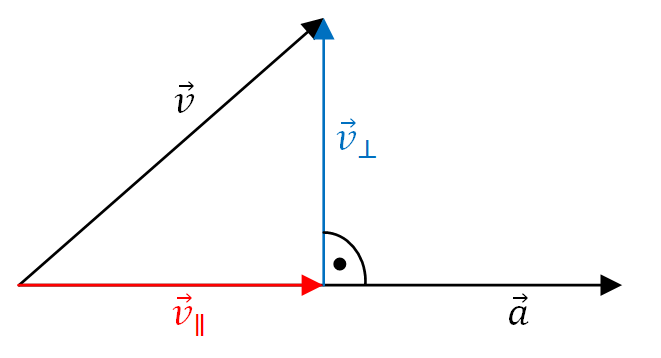
\includegraphics[width=6cm]{pics/1_Projektion.png}
				\end{minipage}
				\begin{minipage}[c]{8cm}
					\begin{equation*} P\vec{a}(\vec{v}) = |\vec{v}|\cdot \cos\alpha = \frac{\vec{a}\bullet \vec{v}}{|\vec{a}|}\end{equation*}
					\begin{equation*} v_{\parallel} = \frac{\vec{a}\bullet \vec{v}}{\vec{a}\cdot \vec{a}}\cdot \vec{a}\end{equation*}
					\begin{equation*} v_{\perp} = \vec{v} - \frac{\vec{a}\bullet \vec{v}}{\vec{a}\cdot \vec{a}}\cdot \vec{a}\end{equation*}
				\end{minipage}
		\end{enumerate}

	\subsubsection{Normalengleichung}
		\begin{equation*}
			\vec{n} \cdot (\vec{a} - \vec{p}) = 0
		\end{equation*}
		Der Normalenvektor $\vec{n}$ steht senkrecht zur Geraden oder zur Ebene. Mit seiner Hilfe und einem Punkt P ($\vec{0P} = \vec{p}$) lässt sich
		die Koordinatengleichung direkt hinschreiben:
		\begin{equation*}
			n_1 + n_2y + n_3z = \vec{n_0} \cdot \vec{p}
		\end{equation*}
		Umgekehrt lässt sich aus der Koordinatengleichung die Normalengleichung herauslesen. \\

		\textbf{Beispiel 1:} Gegebene Punkte: $A=\vektor{2}{2}{-2}$
									 $B=\vektor{3}{-3}{-1})$ \\ \ \\
							 Normale kann mithilfe des Vektorproduktes gefunden werden: \\ \ \\
									 $\vektor{n_1}{n_1}{n_1}\bullet\vektor{2}{2}{-2}=2n_1+2n_2-2n_3$ und
									 $\vektor{n_1}{n_1}{n_1}\bullet\vektor{3}{-3}{-1}=3n_1-3n_2-n_3$\\ \ \\ \ \\
							$\begin{array}{|rrr|r|}
								\hline 
									2 & 2 & -2 & 0 \\
									3 & -3 & -1 & 0 \\
								\hline
							\end{array}$
							$\rightarrow^{...}\rightarrow$	
							$\begin{array}{|rrr|r|}
								\hline 
									1 & 0 & \frac{-2}{3} & 0 \\
									0 & 1 & \frac{-1}{3} & 0 \\
								\hline
							\end{array}$
							$\rightarrow$
							$\vec{n}=\vektor{2}{1}{3}$ für $n_3 = 3$ ($n_3$ ist frei wählbar)\\
	 \textbf{Beispiel 2:} $3x-2y-z=-4\rightarrow\vec{n}=\vektor{3}{-2}{-1}$
		
\subsection{Verhalten zweier Objekte}
	\subsubsection{Schnittwinkel}
		Es wird der spitze Winkel zwischen \ldots{ }berechnet (g, h sind Geraden; E, F Ebenen; m und n Normalen):\\
		\begin{tabular}{llll}
		g $\wedge$ h:
		&$g: \vec{x}=\vec{p}+r\vec{v}$ 
		&$h: \vec{x}=\vec{q}+s\vec{w}$ 
		&$\alpha=\arccos{\frac{|v\bullet w|}{|\vec{v}|\cdot|\vec{w}|}}$\\
		g $\wedge$ h:
		&$g: m_1x+m_2y=b$
		&$h: n_1x+n_2y=c$
		&$\alpha=\arccos{\frac{|m\bullet n|}{|\vec{m}|\cdot|\vec{n}|}}$\\
		g $\wedge$ E:
		&$g: \vec{x}=\vec{p}+r\vec{v}$
		&$E: n_1x+n_2y+n_3z=b$
		&$\alpha=\arcsin{\frac{|v\bullet n|}{|\vec{v}|\cdot|\vec{n}|}}$\\
		E $\wedge$ F:
		&$E: m_1x+m_2y+m_3z=b$
		&$F: n_1x+n_2y+n_3z=c$
		&$\alpha=\arccos{\frac{|m\bullet n|}{|\vec{m}|\cdot|\vec{n}|}}$\\
		\end{tabular}

	\subsubsection{Gegenseitige Lage}
		Es werden jeweils zwei Objekte gleichgesetzt (g, h sind Geraden; E, F
		Ebenen).\\
		\begin{tabular}{lllll}
			&&$g = h$ &$g = E$ &$E = F$\\
			Keine Lösung &$\Rightarrow$ &kollinear oder windschief &parallel
			&parallel\\
			1 Lösung &$\Rightarrow$ &1 Schnittpunkt &1 Schnittpunkt & - \\
			$\infty$ Lösungen (1 Parameter frei wählbar) &$\Rightarrow$ 
			&g und h sind identisch &g liegt in E &1 Schnittgerade ($\vec{n}_E \times \vec{n}_F$) \\
			$\infty$ Lösungen (2 Parameter frei wählbar) &$\Rightarrow$  
			& - & - &E und F sind identisch
		\end{tabular}


\subsection{Orthonormalisierung}
	$\vec{a_1}, \vec{a_2}, \vec{a_3}$ sind linear unabhängig $\longrightarrow \vec{b_1} \bot \vec{b_2} \bot \vec{b_3}$\\
	\begin{minipage}{3cm}
		\begin{equation*}
			\vec{b_1} = \frac{\vec{a_1}}{|\vec{a_1}|}
		\end{equation*}
	\end{minipage}
	\begin{minipage}{5cm}
		\begin{equation*}
			\vec{b_2} = \frac{\vec{a_2} - (\vec{a_2} \bullet \vec{b_1}) \vec{b_1}}{|\vec{a_2} - (\vec{a_2} \bullet \vec{b_1}) \vec{b_1}|}
		\end{equation*}
	\end{minipage}
	\begin{minipage}{5cm}
		\begin{equation*}
			\vec{b_3} = \frac{\vec{a_3} - (\vec{a_3} \bullet \vec{b_1})\vec{b_1} - (\vec{a_3} \bullet \vec{b_2})\vec{b_2}}
					{|\vec{a_3} - (\vec{a_3} \bullet \vec{b_1})\vec{b_1} - (\vec{a_3} \bullet \vec{b_2})\vec{b_2}|}
		\end{equation*}
	\end{minipage} \\ \ \\
	
	\textbf{Beispiel:} $\vec{a_1}=\vektor{1}{0}{0}
						\vec{a_2}=\vektor{1}{1}{0}
						\vec{a_3}=\vektor{1}{1}{1}$ \\
						
						$\vec{b_1}=\frac{\vektor{1}{0}{0}}{\left|\vektor{1}{0}{0}\right|}=\vektor{1}{0}{0}$ \\
						$\vec{b_2}=\frac{\vektor{1}{1}{0}-\left(\vektor{1}{1}{0}\bullet\vektor{1}{0}{0}\right)\vektor{1}{0}{0}}{\left|\vektor{1}{1}{0}-\left(\vektor{1}{1}{0}\bullet\vektor{1}{0}{0}\right)\vektor{1}{0}{0}\right|}=\vektor{1}{1}{0}$\\
						$\vec{b_3}=\frac{\vektor{1}{1}{1}-\left(\vektor{1}{1}{1}\bullet\vektor{1}{0}{0}\right)\vektor{1}{0}{0}-\left(\vektor{1}{1}{1}\bullet\vektor{1}{1}{0}\right)\vektor{1}{1}{0}}{\left|\vektor{1}{1}{1}-\left(\vektor{1}{1}{1}\bullet\vektor{1}{0}{0}\right)\vektor{1}{0}{0}-\left(\vektor{1}{1}{1}\bullet\vektor{1}{1}{0}\right)\vektor{1}{1}{0}\right|}=\vektor{0}{0}{1}$

\subsection{Mittelsenkrechte}
	\begin{equation*}
		\vec{M_{AB}} = \frac{\vec{a} + \vec{b}}{2}
	\end{equation*}

\subsection{Least Squares}
	$A^tAv = A^tb \longrightarrow$ nach $v$ auflösen und den kleinsten Abstand zu bekommen. \qquad $(Av = b)$
		
\subsection{Vektorprodukt/Kreuzprodukt}
	\begin{equation*}
		\vec{c} = \vec{a} \times \vec{b} = \vektor{a_1}{a_2}{a_3} \times \vektor{b_1}{b_2}{b_3} = \left(\begin{array}{c}
			a_2b_3 - a_3b_2\\
			a_3b_1 - a_1b_3\\
			a_1b_2 - a_2b_1
		\end{array}\right)
		=\left(\begin{array}{c}
			\left|\begin{array}{cc}
				a_2 & b_2 \\
				a_3 & b_3 \end{array}\right|\\
			-\left|\begin{array}{cc}
				a_1 & b_1 \\
				a_3 & b_3 \end{array}\right|\\
			\left|\begin{array}{cc}
				a_1 & b_1 \\
				a_2 & b_2 \end{array}\right|
		\end{array}\right)
	\end{equation*}

	\begin{tabular}{ll}
		Zwischenwinkel: &
		\begin{equation*}
			\sin\alpha = \frac{|\vec{a} \times \vec{b}|}{|\vec{a}||\vec{b}|}
		\end{equation*}
	\end{tabular}\\ \\

	Mit Hilfe des Vektorproduktes lässt sich der \textbf{Normalenvektor}
	zweier Vektoren bestimmen. Ausserdem entspricht der Betrag des Vektorproduktes
	dem \textbf{Flächeninhalt} des von den Vektoren $\vec{a}$ und $\vec{b}$
	aufgespannten Parallelogramms. Somit sind $\vec{a}$ und $\vec{b}$ also
	kollinear, wenn $\vec{a}\times\vec{b}=0$. Das Vektorprodukt ist ein
	\textbf{Rechtssystem}
	($\vec{a} \Leftrightarrow$ Daumen; $\vec{b} \Leftrightarrow$ Zeigefinger;
	$\vec{c} \Leftrightarrow$ Mittelfinger). Das Vektorprodukt gilt nur in 3D (im
	Falle eines 2 dimensionalen Systems gilt einfach $a_3 = b_3 = 0$).

	\subsubsection{Algebraische Eigenschaften des Vektorproduktes}
		\begin{tabular}{ll}
			$\vec{a}\times\vec{b} = -(\vec{b}\times\vec{a}) = -\vec{b}\times\vec{a}$
			&(Anti-Kommutativgesetz)\\
			$(r\cdot\vec{a})\times\vec{b} = r(\vec{a}\times\vec{b}) = \vec{a}\times(r\cdot\vec{b})$
			&(gemischtes Assoziationsgesetz)\\
			$(\vec{a}+\vec{b})\times\vec{c} = (\vec{a}\times\vec{c})+(\vec{b}\times\vec{c})
			= \vec{a}\times\vec{c}+\vec{b}\times\vec{c}$\\
			$\vec{a}\times(\vec{b}+\vec{c}) = (\vec{a}\times\vec{b})+(\vec{a}\times\vec{c})
			= \vec{a}\times\vec{b}+\vec{a}\times\vec{c}$ &(Distributivgesetz)
		\end{tabular}
	
	\subsubsection{Volumen eines Parallelpipeds}
		\begin{equation*}
			det(A) = |\vec{a}; \vec{b}; \vec{c}| = (\vec{a} \times \vec{b}) \bullet \vec{c} = a_1b_2c_3 + a_2b_3c_1 + a_3b_1c_2 - c_1b_2a_3 - c_2b_3a_1 - c_3b_1a_2
		\end{equation*}

		$|\vec{a}; \vec{b}; \vec{c}| = 0 \Leftrightarrow \vec{a}; \vec{b}; \vec{c}$ komplanar \qquad 
		$|\vec{a}; \vec{b}; \vec{c}| > 0 \Leftrightarrow \vec{a}; \vec{b}; \vec{c}$ bilden Rechtssystem \qquad
		$|\vec{a}; \vec{b}; \vec{c}| < 0 \Leftrightarrow \vec{a}; \vec{b}; \vec{c}$ bilden Linkssystem

	\subsubsection{Anwendung}
		Abstand Punkt/Ebene, Gerade/Gerade:
		\begin{equation*}
			d = (\vec{p_1} - \vec{p_2}) \cdot \vec{n_0} = (\vec{p_1} - \vec{p_2}) \cdot \frac{\vec{r_1} \times \vec{r_2}}{|\vec{r_1} \times \vec{r_2}|}
		\end{equation*} 

		Abstand Punkt/Gerade:
		\begin{equation*}
			d = \frac{\vec{r} \times (\vec{p} - \vec{p_0})}{|\vec{r}|}
		\end{equation*}



























